\section{Scaling laws for judges}
\label{sec:scaling}

% Provenance: experiment 31 (free CPU re-analysis of the saved results of experiments 26, 28 and 29; no model calls).
If a judge is an ordinary learning problem, its held-out loss should fall with data the way other losses do.
We fit a saturating power law to the saved learning curves of experiments 26, 28 and 29,
\begin{equation}
\mathrm{error}(N)=\mathrm{floor}+a\,(N/N_{\min})^{-b},
\label{eq:scaling}
\end{equation}
where $N$ is the number of human ratings spent on fitting, $a$ is the excess at the smallest $N$ tested, $b\in[0.02,3]$ and $\mathrm{floor},a\ge0$.
The scaling-law literature~\citep{kaplan2020scaling,hoffmann2022training} treats cross-entropy as the quantity that falls smoothly with data, so we ask whether the curves of a CE-fit judge follow Equation~\eqref{eq:scaling} and whether those of a Pearson-fit judge do.
We fit by weighted least squares with weights $1/\mathrm{SE}^2$ from the saved standard errors, exactly over a grid of 150 values of $b$, and take percentile 95\% intervals from 2{,}000 parametric bootstrap draws per curve.
A curve is non-monotone if any step up exceeds 1.96 standard errors, flat if it declines by under two standard errors, and poorly fit if the root-mean-square residual exceeds 10\% of its range; its floor is not identified if the floor's interval is wider than that range.
We do not fit curves with three budgets.

\begin{figure*}[t]
\centering
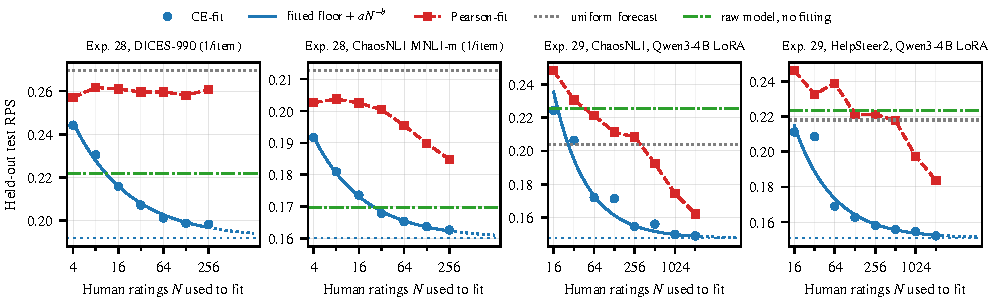
\includegraphics[width=\textwidth]{figures/fig_scaling.pdf}
\caption{\textbf{CE curves saturate with the number of human ratings in most panels; Pearson curves are flat or still falling at the largest budget.}
Held-out ranked probability score (RPS) against the number of human ratings, with a saturating power-law fit for the CE-fit judge.
Vertical axis: held-out test RPS (0--1; lower is better); horizontal axis: number of human ratings $N$ used to fit (log scale).
Left two panels: frozen frontier judges with a 27-setting head, mean over five judges, one rating per item, on DICES-990 and ChaosNLI MNLI-matched (experiment 28).
Right two panels: raw (uncalibrated) forecasts of CE-trained and Pearson-trained LoRA judges, Qwen3-4B-Instruct on ChaosNLI and HelpSteer2 (experiment 29; 10 draws per budget).
Blue: CE-fit or CE-trained, with the fitted $\mathrm{floor}+aN^{-b}$ (solid over the tested range, dotted beyond it); red dashed: Pearson-fit or Pearson-trained; dotted: uniform; dash-dotted green: the untuned model.
The CE judge is chosen by minimizing training cross-entropy within its family (exhaustive search for the head; AdamW with a validation-selected checkpoint for LoRA); the Pearson judge is chosen the same way with correlation as objective.
No interval is drawn (fits with intervals: \Cref{tab:scaling}).}
\label{fig:scaling}
\end{figure*}

\paragraph{CE curves usually follow a saturating power law.}
Equation~\eqref{eq:scaling} fits the CE curve in 9 of the 11 panels; \Cref{tab:scaling} in \appref{app:extra} lists every panel, its fit verdict and its floor.
For the frozen judges of experiment 28 with one rating per item, it fits all 25 judge-by-dataset cells on RPS but identifies the floor in only 8.
Where the floor is identified, the median exponent is $0.66$ for RPS (8 of 25 cells), $0.82$ for cross-entropy (20 of 25) and $0.59$ for total variation distance (10 of 25).
For CE-trained LoRA on the three experiment 29 panels with eight budgets, $b$ is $0.89$ (95\% interval $[0.76,0.99]$) on ChaosNLI with Qwen3-4B, where the law fits; the other two panels have $b$ of $0.76$ and $0.64$ but residuals above the 10\% rule (\Cref{tab:scaling}).

\paragraph{Pearson curves rarely do.}
Equation~\eqref{eq:scaling} fits the Pearson curve in one of the eleven panels, ChaosNLI with Qwen3-4B, with $b=0.09$ and an extrapolated floor of $0.002$, which is implausible when raters disagree.
Eight Pearson curves fit poorly and two are flat (DICES-990 stays at RPS $0.26$ against $0.27$ for uniform).
All 25 judge-by-dataset cells with five ratings per item are non-monotone.
At the largest $N$ tested, the Pearson-fit RPS lies above the CE-fit floor in 20 of 25 experiment 28 cells with one rating per item at a 95\% bound (cross-entropy: 25 of 25; TVD: 21 of 25), so the Pearson curve has not reached where the CE curve saturates and the data cannot say whether it does.
The result concerns these two objectives in these families, not every correlation objective with every optimizer.

\paragraph{What we cannot say.}
The fits are indications, not laws.
The saved standard errors are approximate, and those of experiment 26 are too wide to identify any law; we estimate no human leave-one-vote-out floor; nothing is observed beyond 320 ratings (experiments 26 and 28) or $2{,}048$ (experiment 29), so the dotted extrapolations in \Cref{fig:scaling} are extrapolations; and the exponents describe five rating sets, two model families and two training methods.
\appref{app:extra-tables} lists every caveat.
